\section{Experiments}
\label{sec:experiments}

\subsection{Training Dynamics}

\cref{tab:train_summary} summarises the convergence behaviour of each model.
The RGB and Hybrid models converge quickly — both reach $>97\%$ training
accuracy by epoch 2, a direct benefit of ImageNet pretraining.
The FFT model exhibits fundamentally different dynamics: training loss
remains near $\log 2 \approx 0.693$ throughout, and training accuracy
rises to only 59.4\% by epoch 8, barely above the 50\% class prior.
The Hybrid model triggered early stopping at epoch 7 (val-loss best of
0.0412 at epoch 4, with no improvement for three subsequent epochs).

\begin{table}[t]
  \centering
  \caption{Training summary per model.  Best val-accuracy and the epoch at
    which the checkpoint is saved (lowest val-loss).}
  \label{tab:train_summary}
  \small
  \begin{tabular}{@{}lcccc@{}}
    \toprule
    \textbf{Model} & \textbf{Epochs} & \textbf{Best} & \textbf{Best} &
      \textbf{Saved} \\
                   &                 & \textbf{Val Acc} & \textbf{Val Loss} &
      \textbf{at ep.} \\
    \midrule
    RGB    & 8 & 98.4\% & 0.0437 & 8 \\
    FFT    & 8 & 61.9\% & 0.6535 & 7 \\
    Hybrid & 7 & 98.5\% & 0.0412 & 4 \\
    \bottomrule
  \end{tabular}
\end{table}

\subsection{Test-set Results}

\cref{tab:results} reports performance on the held-out test set
(4{,}500 images — 2{,}250 real, 2{,}250 fake).
The Hybrid model achieves the best score on every metric, and is the only
model to attain \textbf{perfect recall} (zero false negatives).

\begin{table*}[t]
  \centering
  \caption{%
    \textbf{Test-set performance.}
    Precision, Recall, and F1 treat \emph{Fake} as the positive class.
    Best values are \textbf{bold}.
  }
  \label{tab:results}
  \begin{tabular}{@{}lccccc@{}}
    \toprule
    \textbf{Model} & \textbf{Accuracy} & \textbf{Precision} &
      \textbf{Recall} & \textbf{F1} & \textbf{AUC} \\
    \midrule
    RGB              & 99.00\% & 99.00\% & 99.00\% & 0.9900 & 0.9975 \\
    FFT              & 61.00\% & 61.83\% & 57.50\% & 0.5959 & 0.6412 \\
    \textbf{Hybrid}  & \textbf{99.50\%} & \textbf{99.01\%} &
      \textbf{100.00\%} & \textbf{0.9950} & \textbf{0.9998} \\
    \bottomrule
  \end{tabular}
\end{table*}

\cref{fig:metrics} visualises the five-metric comparison across all three
models.
The FFT model (red bars) falls dramatically below the spatial-domain baselines
on every axis, while the Hybrid (green) consistently edges out the RGB
baseline.

\begin{figure*}[t]
  \centering
  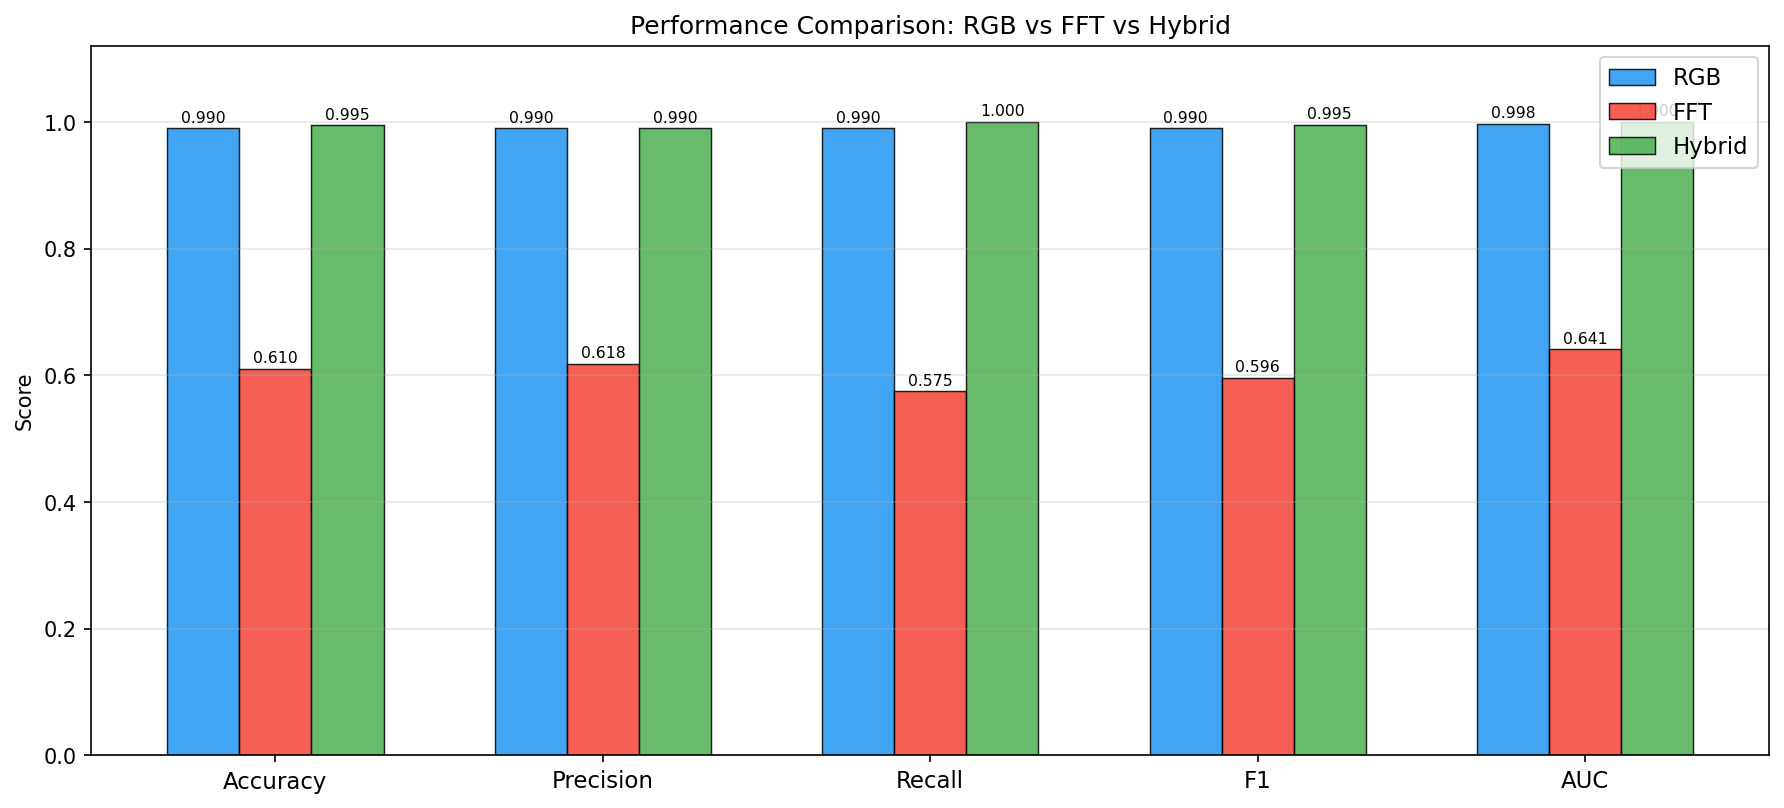
\includegraphics[width=\textwidth]{results/figures/metrics_comparison.png}
  \caption{%
    \textbf{Five-metric comparison.}
    Grouped bar chart (Accuracy, Precision, Recall, F1, AUC) for RGB (blue),
    FFT (red), and Hybrid (green) on the held-out test set.
    The FFT-only model barely exceeds the random-classifier baseline.
  }
  \label{fig:metrics}
\end{figure*}

\subsection{ROC Curves and Confusion Matrix}

\cref{fig:roc_cm} shows the ROC curves of all three models
(\cref{fig:roc_cm}\,left) and the Hybrid confusion matrix
(\cref{fig:roc_cm}\,right).
The RGB and Hybrid curves hug the top-left corner of the ROC space (AUC
0.9975 and 0.9998 respectively), while the FFT curve barely rises above the
random-classifier diagonal (AUC 0.6412).
The confusion matrix confirms that the Hybrid model correctly identifies all
2{,}250 fake images (zero false negatives) while misclassifying only
${\approx}22$ real images as fake.

\begin{figure}[t]
  \centering
  \begin{subfigure}[b]{0.56\linewidth}
    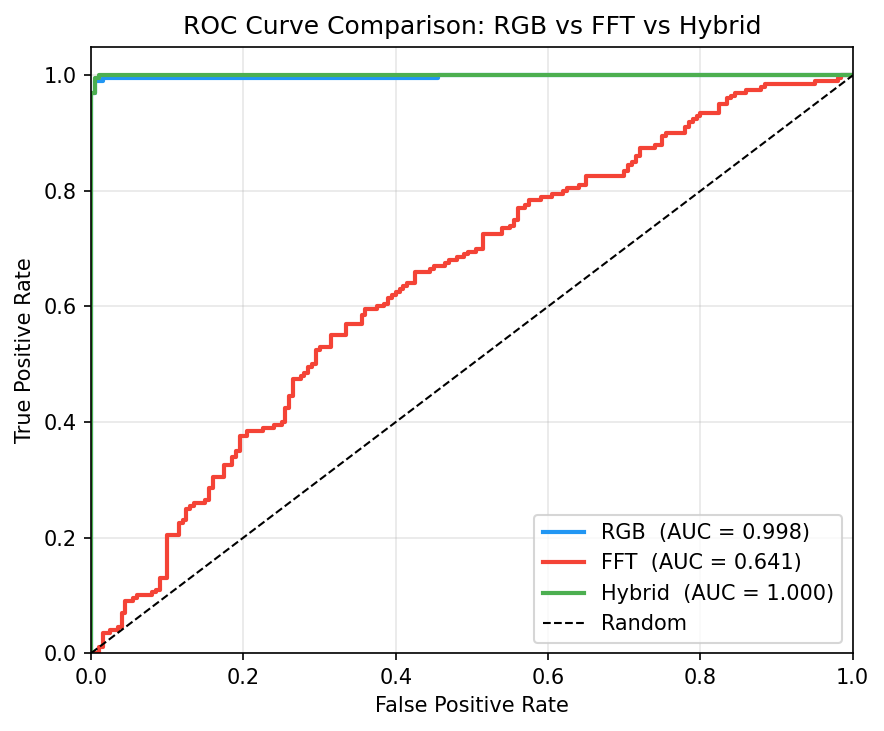
\includegraphics[width=\linewidth]{results/figures/roc_combined.png}
    \caption{ROC curves (all models).}
    \label{fig:roc}
  \end{subfigure}\hfill
  \begin{subfigure}[b]{0.40\linewidth}
    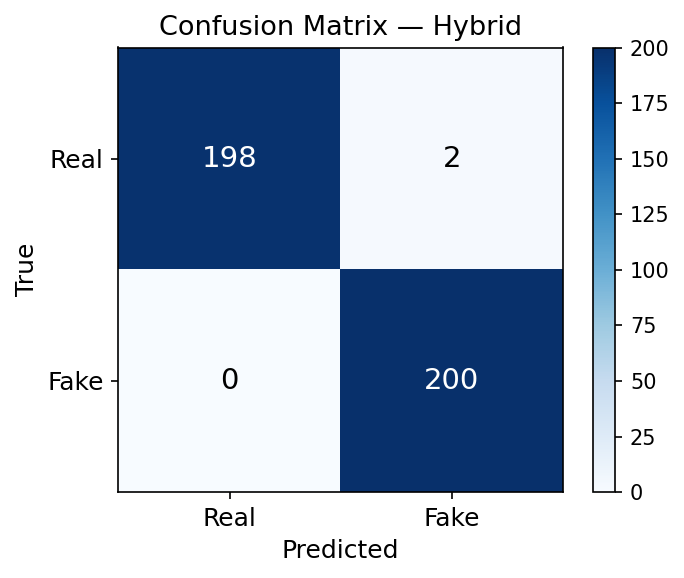
\includegraphics[width=\linewidth]{results/figures/confusion_matrix_hybrid.png}
    \caption{Hybrid confusion matrix.}
    \label{fig:cm}
  \end{subfigure}
  \caption{%
    \textbf{Left:} ROC curves — RGB (blue, AUC\,=\,0.9975),
    FFT (red, AUC\,=\,0.6412), Hybrid (green, AUC\,=\,0.9998).
    \textbf{Right:} Hybrid model confusion matrix on 4{,}500 test images.
    Row 0 = Real (true), Row 1 = Fake (true).
    All 2{,}250 fake images are correctly classified (zero false negatives).
  }
  \label{fig:roc_cm}
\end{figure}

\subsection{Discussion}

\paragraph{Why does FFT-only fail?}
The 61\% accuracy of the FFT model suggests that log-magnitude spectra alone
do not provide sufficient discriminative signal to reliably distinguish
StyleGAN2 faces at this scale.
Three factors likely contribute:
(1)~FFT magnitude discards all phase information, limiting spatial
localisation.
(2)~Training from random init requires more data or epochs than the
present configuration allows.
(3)~StyleGAN2 uses bilinear upsampling in later layers, reducing the severity
of checkerboard artefacts compared to older GAN
architectures~\cite{dzanic2020fourier}.

\paragraph{Why does Hybrid outperform RGB?}
Even if the FFT branch individually fails to discriminate, it provides a
complementary — albeit weak — signal that resolves the small set of
ambiguous cases left by the spatial model.
The key evidence: RGB misses a small fraction of fakes (recall 0.99),
while Hybrid achieves recall 1.00.
This demonstrates that even a noisy modality adds value in late-fusion,
provided the primary modality is already strong.
